\subsection[Ordinal response]{Ordinal Response: Proportional Odds Model}%
\label{sec:ordinal}
\ix{proportional odds model|(}
The proportional odds model extends logistic regression to handle an
ordinal response variable.  For example, the response variable \pname{improve} in
the arthritis data actually has 3 levels, corresponding to None,
Some, or Marked improvement.

\begin{table}[htb]
 \caption{Arthritis data: Response frequencies and adjacent category logits}\label{tab:arthlogit2}
 \begin{center}
 \begin{tabular}{ll | rrr | r| rr}
 \hline
      &           & \multicolumn{3}{c|}{Improvement} & \\
  Sex & Treatment & None & Some & Marked & Total & $L_1$ & $L_2$ \\ \hline
% 
  F & Active & 6 & 5 & 16 & 27 & -1.253 & -0.375 \\ 
  F & Placebo & 19 & 7 & 6 & 32 & 0.379 & 1.466 \\[2mm]
%
  M & Active & 7 & 2 & 5 & 14 & 0.000 & 0.588 \\ 
  M & Placebo & 10 & 0 & 1 & 11 & 2.302 & 2.302 \\ 
 \hline
 \end{tabular}
 \end{center}
\end{table}

One way to model these data is to consider two logits for the
dichotomies between adjacent categories:
\begin{equation*}
  L_1
 = \log  \frac{ \pi_{ij1} } { \pi_{ij2}  +  \pi_{ij3} }
 = \mbox{logit ( None vs. [Some or Marked] )}
  \]
  \[
  L_2
 = \log  \frac{ \pi_{ij1}  +  \pi_{ij2} } { \pi_{ij3} }
 = \mbox{logit ( [None or Some] vs. Marked)}
\end{equation*}

\tabref{tab:arthlogit2} shows the data and the sample estimates
of the adjacent category logits.  For example, for males given the
active treatment, $L_1 = \log (7/7) = 0$, and
$L_2 = \log (9/5) = 0.588$.
Consider a linear logistic regression model for each logit:
\begin{equation} \label{eq:logod1}
  L_1
 = \alpha _1  +  \vec{x}_{ij}\trans \,  \vec{\beta} _1
  \end{equation}
  \begin{equation} \label{eq:logod2}
  L_2
 = \alpha _2  +  \vec{x}_{ij}\trans \,  \vec{\beta} _2
\end{equation}

\begin{figure}[htb]
  \centering
  \includegraphics[scale=.7]{ch6/fig/podds}
  \caption[Proportional odds model]{Proportional odds model.  The model
assumes that the regression functions for different response
categories are parallel on the logit scale.}\label{fig:podds}
\end{figure}
The proportional odds assumption is that
\boldital{the regression functions are parallel} on the logit scale,
i.e., that
\(\vec{\beta}_1 = \vec{\beta} _2\),
as illustrated in \figref{fig:podds} for a four-category response.

For the arthritis example, with additive effects for sex and
treatment on both log odds, the proportional odds model is
\begin{equation} \label{eq:logst1}
  L_1 = \alpha _1  +
  \beta _1 \,  x_1  +
  \beta _2 \,  x_2
\end{equation}
\begin{equation} \label{eq:logst2}
  L_2 = \alpha _2  +
  \beta _1 \,  x_1  +
  \beta _2 \,  x_2
\end{equation}
where:
\begin{itemize}

\item \(x_1\) and \(x_2\) are dummy variables representing sex and
       treatment.

\item \(\alpha _1\) is the log odds of no improvement (vs.\  some or
       marked) for males receiving the placebo.

\item \(\alpha _2\) is the log odds of no improvement or some
       improvement (vs.\  marked) for males receiving the placebo.

\item \(\beta _1\) is the increment to \emph{both} log odds for being
       female.  Therefore, \(e^{ \beta _1 }\) gives the odds of
       improvement for females relative to males.

\item \(\beta _2\) is the increment to both log odds for being in the
       active treatment group.  \(e^{ \beta _2 }\) gives the odds of
       improvement for the active treatment group relative to
       placebo.

\end{itemize}

The corresponding models including effects of age, as well as
treatment and sex are similar to \eqref{eq:logst1} and \eqref{eq:logst2}, with the addition of
a term $\beta _3$  age.

\subsection{Plotting results from \PROC{LOGISTIC}}

Plotting results for the proportional odds model is similar to the
earlier examples (e.g., \secref{sec:logist-quantp})
for a binary response variable%
\glosstex{binary}.  The main differences for a polytomous response are:

\begin{itemize}

\item The validity of the analysis depends on the correctness of the
       proportional odds assumption.  A test of this assumption
       appears in the output from \PROC{LOGISTIC}.

\item The results from \PROC{LOGISTIC} are cast in terms of predicted
       probabilities and fitted logits for response \emph{less than}
       each of the cutpoints.  To plot Pr\{Improve\}, we must reverse
       the sense of the probabilities and logits.

\end{itemize}

\begin{Example}[arthrit12]{Arthritis treatment}
This example fits the effects of treatment,
sex and age for the proportional odds model with the arthritis data.
Note that the dependent variable is \pname{improve}, with values 0, 1,
and 2.
%% \inclsas{glogist2)
%% \input{glogis2a} %% level: 3

\begin{listing}
   *-- Proportional Odds Model: Effects of treat, sex and age;
proc logistic data=arthrit nosimple;
   model  improve = _sex_  _treat_ age ;
   output out=results p=predict l=lower u=upper
                      xbeta=logit stdxbeta=selogit / alpha=.33;
\end{listing}

The response profile,
shown in \outref{out:glogist2.1}, displays the ordering of the outcome variable.
Note that logits are formed from top to bottom, i.e., none vs.\  some
or marked, none or some vs.\  marked.  The output (``Score test'')
also shows the
proportional odds assumption is reasonable here.
\begin{Output}[htb]
\caption{Proportional odds model: Response profiles and score test}\label{out:glogist2.1}
\begin{output}
                          Response Profile
                     Ordered
                       Value  IMPROVE     Count

                           1        0        42
                           2        1        14
                           3        2        28

          Score Test for the Proportional Odds Assumption

              Chi-Square = 2.4917 with 3 DF (p=0.4768)
\end{output}
\end{Output}

The parameter estimates
for the model \eqref{eq:logst1}-\eqref{eq:logst2} appear in
\outref{out:glogist2.2}.
These values relate to the odds of a poorer response (they
are all negative).

\begin{Output}[htb]
\caption{Proportional odds model: Parameter estimates}\label{out:glogist2.2}
\begin{output}
              Analysis of Maximum Likelihood Estimates

             Parameter  Standard     Wald        Pr >    Standardized
   Variable   Estimate    Error   Chi-Square  Chi-Square   Estimate

   INTERCP1     3.7837    1.1530     10.7683      0.0010            .
   INTERCP2     4.6827    1.1949     15.3569      0.0001            .
   _SEX_       -1.2517    0.5321      5.5343      0.0186    -0.317412
   _TREAT_     -1.7453    0.4772     13.3770      0.0003    -0.483871
   AGE         -0.0382    0.0185      4.2358      0.0396    -0.268666
\end{output}
\end{Output}

The \ODS\ \pname{RESULTS} contains, for each observation, the
predicted probability, Pr\{Not Improved\} and estimated logit for both
types of odds.  These are distinguished by the variable
\verb|_LEVEL_|.  To plot probabilities for both types of improvement in a
single graph, the values of \pname{TREAT} and \verb|_LEVEL_| are combined
in a single variable.  To plot Pr\{Improve\}, we must reverse the
direction of the variables in a data step:
%% \inclsas{glogist2)
%% \input{glogis2b} %% level: 3

\begin{listing}
data results;
   set results;
   treatl = treat||put(_level_,1.0);
   if _level_=0 then better = (improve > 0);
                else better = (improve > 1);
   *-- Change direction of probabilities \& logit;
   predict = 1 - predict;
   lower = 1 - lower;
   upper = 1 - upper;
   logit = -logit;
\end{listing}

The first few observations in the \Dset\ \pname{RESULTS} after these
changes are shown below:

\begin{output}
   ID  TREAT   SEX IMPROVE _LEVEL_ PREDICT   LOWER   UPPER   LOGIT

   57 Treated Male    1       0      0.267   0.417   0.157  -1.008
   57 Treated Male    1       1      0.129   0.229   0.069  -1.907
    9 Placebo Male    0       0      0.085   0.149   0.048  -2.372
    9 Placebo Male    0       1      0.037   0.069   0.019  -3.271
   46 Treated Male    0       0      0.283   0.429   0.171  -0.932
   46 Treated Male    0       1      0.138   0.238   0.076  -1.831
     ...
\end{output}

As in the earlier examples, an \ADS\ is used to add more
descriptive labels and confidence intervals to the plots.  (This adds
somewhat more work, but I prefer the plots labeled this way, rather
than with legends at the bottom.)
%% \inclsas{glogist2)
%% \input{glogis2c} %% level: 3

\begin{listing}
proc sort data=results;
   by sex treatl age;
data bars;
   set results;
   by sex treatl;
   length text$8;
   xsys='2'; ysys='2';
   if treat='Placebo' then color='BLACK';
                      else color='RED';
   x  = age; line=33;
   *-- plot confidence limits  ;
   y  = upper;  function='MOVE   '; output;
   text='-';    function='LABEL  '; output;
   y  = lower;  function='DRAW   '; output;
   text='-';    function='LABEL  '; output;
   if last.treatl then do;
      y = predict;
      x = age+1; position='C'; size=1.4;
      text = treat; function='LABEL'; output;
      position='F';
      if _level_ = 0
         then text='> None';
         else text='> Some';
      output;
      end;
   if first.sex then do;
      ysys ='1'; y=90;
      xsys ='1'; x=10; size=1.5;
      text = sex; function='LABEL'; output;
      end;
\end{listing}
The \PROC{GPLOT} step below gives the two plots shown side-by-side
in \figref{fig:glogist2}.
\begin{listing}
goptions hby=0;
proc gplot;
   plot predict * age = treatl / vaxis=axis1 haxis=axis2
                                nolegend anno=bars    ;
   by sex;
   axis1 label=(h=1.4 a=90 'Prob. Improvement (67% CI)')
         value=(h=1.2) order=(0 to 1 by .2);
   axis2 label=(h=1.4)
         value=(h=1.2) order=(20 to 80 by 10)
         offset=(2,5);
   symbol1 v=+ h=1.4 i=join l=3 c=black;
   symbol2 v=+ h=1.4 i=join l=3 c=black;
   symbol3 v=$ h=1.4 i=join l=1 c=red;
   symbol4 v=$ h=1.4 i=join l=1 c=red;
\end{listing}

\begin{figure}[htb]
 \begin{minipage}[t]{.49\linewidth}
  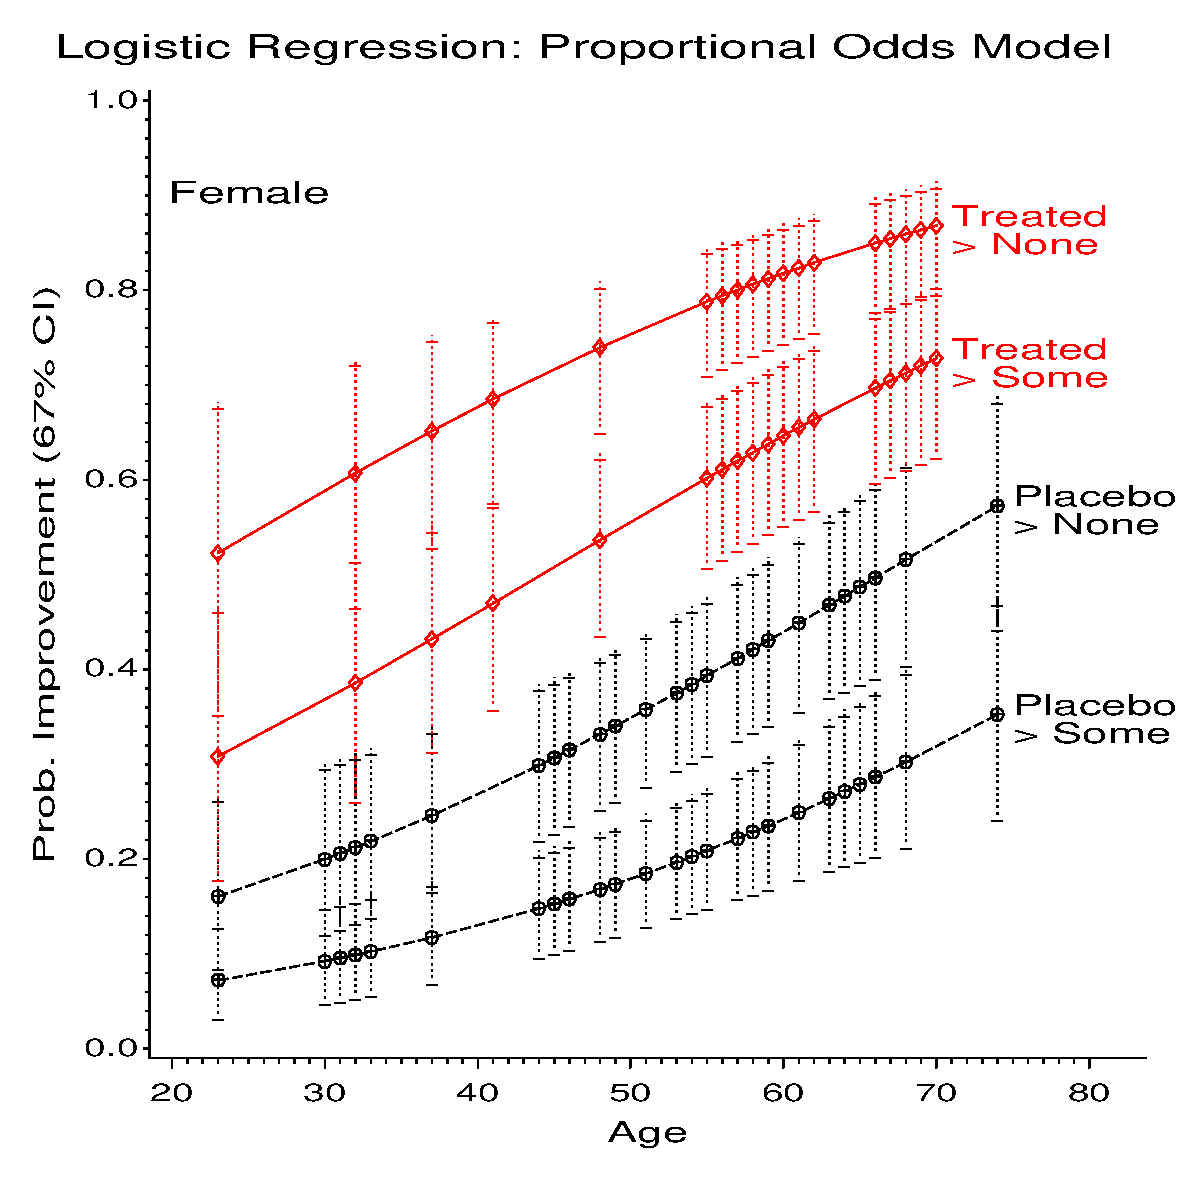
\includegraphics[width=1\linewidth]{ch6/fig/glogist22}
 \end{minipage}%
 \hfill
 \begin{minipage}[t]{.49\linewidth}
  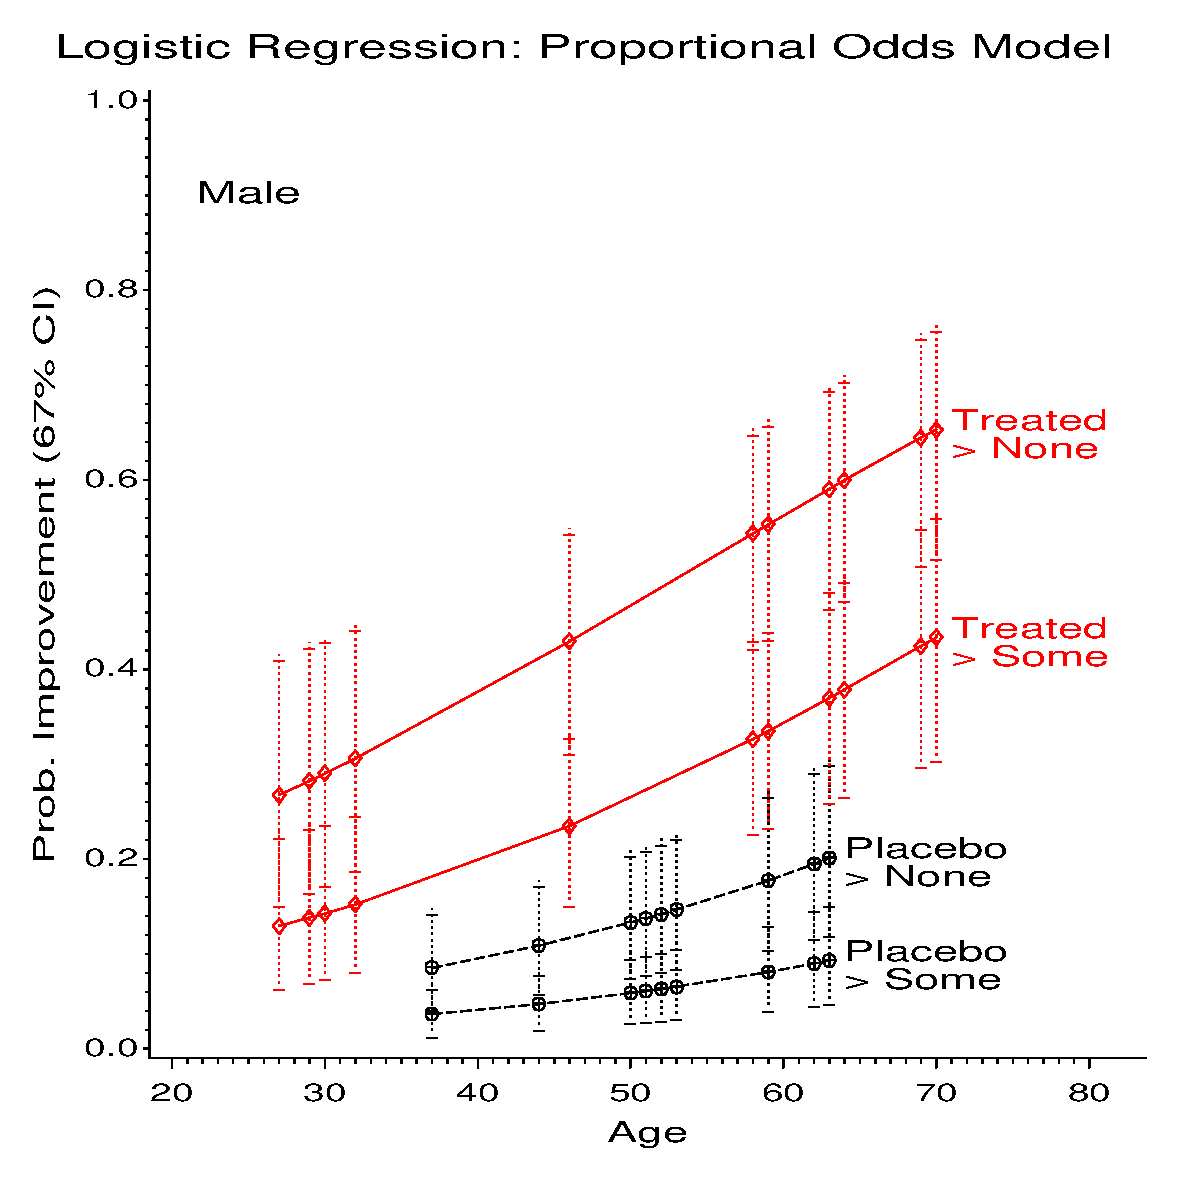
\includegraphics[width=1\linewidth]{ch6/fig/glogist23}
 \end{minipage}
  \caption[Predicted probabilities for the proportional odds model]{Predicted probabilities for the proportional odds model.
  For each group, the curve labeled $>$None gives predicted probabilities for a response of Some or Marked improvement; the curve labeled $>$Some gives that for a response of Marked improvement.}\label{fig:glogist2}
\end{figure}
\ix{proportional odds model|)}
\end{Example}
